\chapter{Implementacja drzewa \emph{Patricia}}\label{cha:czescPraktyczna}

    Zgodnie z celem jaki postawiliśmy sobie w tej pracy, poddaliśmy wnikliwej analizie wszystkie algorytmy dotyczące drzew \emph{Trie} opisane przez Knuth'a w jego książce w~rozdziale ,,6.3. Wyszukiwanie Cyfrowe`` (ang. \emph{Digital Searching}). Aby dobrze zrozumieć zasady ich działania i dokładnie opisać je w swojej pracy postanowiliśmy przetestować swoje podejrzenia, tworząc pierwszą iterację implementacji drzewa \emph{Patricia}. 
	
    Pierwszą wersję implementacji wykonaliśmy według algorytmu opisanego w sekcji dotyczącej drzewa \emph{Patricia}~\ref{sec:DrzewoPatricia}. Celem było stworzenie implementacji, której rezultatem będzie taka sama struktura, jaką Knuth opisuje w swojej książce. Aby to osiągnąć, stworzyliśmy klasę symulującą reprezentację binarną maszyny \emph{MIX} oraz oddzielną klasę symulującą kodowanie znaków odpowiadającą tej z maszyny \emph{MIX}. Napisaliśmy dla niej serię testów, która pozwalała -- metodą prób i błędów -- modyfikować implementację oraz dociekać prawidłowego toku rozwoju implementacji.
    
    Wprowadzając zmiany do implementacji, testując poprawność działania algorytmów i rozjaśniając nieścisłości lub trudne do zrozumienia koncepcje opisane w książce źródłowej, zdobyliśmy wiedzę pozwalającą na szczegółowe opisanie tych algorytmów w niniejszej pracy. Powtarzając wielokrotnie ten proces udało się nam osiągnąć implementację zgodną z opisem Knuth'a oraz -- wprowadzając pewne modyfikacje -- naszą autorską wersję.
    
    To wszystko nie byłoby możliwe bez stworzenia i zastosowania ogromnej ilości testów jednostkowych. Pod koniec pracy nad programem zbiór testujący zawierał 570 złożonych testów, gdzie każdy z nich składał się z wielu porównań (ang. \emph{assert(s)}). 
    
    Rysunek~\ref{fig:Tests} przedstawia wynik oraz czas testowania programu.
    
    \begin{figure}
		\caption{Przykładowy wynik wykonania wszystkich testów zawartych w programie projektowym. Obrazek przedstawia fragment konsoli środowiska oprogramowania o nazwie \emph{IntelliJ IDEA}, w którym pisaliśmy oraz testowaliśmy program projektowy. }\label{fig:Tests}
		\centering
		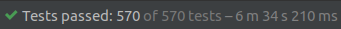
\includegraphics[width = 0.5\textwidth]{tests.png}
	\end{figure}

    Długi czas wykonywania testów wynika z przetwarzania dwóch, dużych plików. Jeden z nich ma rozmiar 8,4MB, a drugi 1,5MB. Obydwa zawierają dane wejściowe w~formacie \emph{DIMACS CNF}. 
	
	\section{Wyzwania implementowania w języku programowania \emph{Java}}\label{sec:AlgorytmPRozszerzenieTworzenieWstawienieDodawanieUwagi}
		
		Należy zwrócić szczególną uwagę na fakt, iż Knuth w swoim tłumaczeniu zakłada iteracje po indeksach zaczynających się od 1, podczas gdy \emph{Java} naturalnie przyjmuje indeksowanie od 0. W związku z tym należy dostosować algorytm tak, by brał to pod uwagę. W efekcie nasza implementacja drzewa \emph{Patricia} przyjmuje postać przedstawioną na rysunku~\ref{fig:PatriciaTreeJavaImplementation}.
		
		\begin{figure}[htb]
			\caption{Schemat drzewa \emph{Patricia} stworzonego przez implementacje w języku \emph{Java} w zgodności z algorytmem opisanym przez Knuth'a w ,,Sztuka programowania tom 3''~\cite{KnuthsTheArtOfComputerProgramming3}. Obrazuje przesunięcie pozycji klucza w pliku spowodowaną różnicą początkowego indeksu. Różnice można zauważyć porównując tę figurę względem figury~\ref{fig:PatriciaTree}.}\label{fig:PatriciaTreeJavaImplementation}
			\centering
			\begin{tikzpicture}[
			>={Stealth[inset=0pt,length=4pt, angle'=45,round]},
			nodeBox/.style = { rectangle, top color = white, bottom color = white, draw, black, text = black, minimum width = 1.25 cm, minimum height = 1.25 cm, font = \scriptsize, inner sep=0.05cm, outer sep=0.05cm },
			word/.style = { font = \scriptsize, inner sep=0.5pt, outer sep=0.5pt, text = black },
			greekSymbol/.style = { ellipse, minimum width = 0.5 cm, minimum height = 0.5 cm, fill, color = black, font = \small, inner sep=0pt, outer sep = 0pt, text = white },
			position/.style = { ellipse, minimum width = 0.5 cm, minimum height = 0.5 cm, top color = white, bottom color = white, draw, black, font = \scriptsize, inner sep=0pt, outer sep = 0pt, text = black}
			]
			
			\def\oneUnit{1.25cm}
			
			\node[nodeBox] (THISskip) at (-2*\oneUnit,1*\oneUnit) {$0$};
			\node[greekSymbol] (THISsymbol) at (-2.3*\oneUnit, 1.3*\oneUnit) {$0$};
			\node[position] (THISposition) at (-1.7*\oneUnit, 1.3*\oneUnit) {0};
			\node[word] (THIS) at (-2*\oneUnit, 0.65*\oneUnit) {(\texttt{THIS})};
			
			
			
			\node[nodeBox] (ISskip) at (-4*\oneUnit,-1*\oneUnit) {$0$};
			\node[greekSymbol] (ISsymbol) at (-4.3*\oneUnit, -0.7*\oneUnit) {$1$};
			\node[position] (ISposition) at (-3.7*\oneUnit,-0.7*\oneUnit) {5};
			\node[word] (IS) at (-4*\oneUnit, -1.35*\oneUnit) {(\texttt{IS})};
			
			
			
			\node[nodeBox] (BUILTskip) at (-7.5*\oneUnit,-3*\oneUnit) {$1$};
			\node[greekSymbol] (BUILTsymbol) at (-7.8*\oneUnit, -2.7*\oneUnit) {$6$};
			\node[position] (BUILTposition) at (-7.2*\oneUnit,-2.7*\oneUnit) {28};
			\node[word] (BUILT) at (-7.5*\oneUnit, -3.35*\oneUnit) {(\texttt{BUILT})};
			
			\node[nodeBox] (THEskip) at (-0.5*\oneUnit,-3*\oneUnit) {$11$};
			\node[greekSymbol] (THEsymbol) at (-0.8*\oneUnit, -2.7*\oneUnit) {$2$};
			\node[position] (THEposition) at (-0.2*\oneUnit,-2.7*\oneUnit) {8};
			\node[word] (THE) at (-0.5*\oneUnit, -3.35*\oneUnit) {(\texttt{THE})};
			
			
			
			\node[nodeBox] (JACKskip) at (-6*\oneUnit,-5*\oneUnit) {$2$};
			\node[greekSymbol] (JACKsymbol) at (-6.3*\oneUnit, -4.7*\oneUnit) {$5$};
			\node[position] (JACKposition) at (-5.7*\oneUnit,-4.7*\oneUnit) {23};
			\node[word] (JACK) at (-6*\oneUnit, -5.35*\oneUnit) {(\texttt{JACK})};
			
			\node[nodeBox] (THATskip) at (-2*\oneUnit,-5*\oneUnit) {$1$};
			\node[greekSymbol] (THATsymbol) at (-2.3*\oneUnit, -4.7*\oneUnit) {$4$};
			\node[position] (THATposition) at (-1.7*\oneUnit,-4.7*\oneUnit) {18};
			\node[word] (THAT) at (-2*\oneUnit, -5.35*\oneUnit) {(\texttt{THAT})};
			
			
			
			\node[nodeBox] (HOUSEskip) at (-7.5*\oneUnit,-7*\oneUnit) {$1$};
			\node[greekSymbol] (HOUSEsymbol) at (-7.8*\oneUnit, -6.7*\oneUnit) {$3$};
			\node[position] (HOUSEposition) at (-7.2*\oneUnit,-6.7*\oneUnit) {12};
			\node[word] (HOUSE) at (-7.5*\oneUnit, -7.35*\oneUnit) {(\texttt{HOUSE})};
			
			\draw [->] (THISskip) -- node[yshift = -0.25*\oneUnit, xshift = -0.5*\oneUnit] {\tiny $0$} ++ (-2*\oneUnit, 0*\oneUnit) -- (ISskip);
			
			\draw [->] (ISskip) -- node[yshift = -0.25*\oneUnit, xshift = -1.25*\oneUnit] {\tiny $0$} ++ (-3.5*\oneUnit, 0*\oneUnit) -- (BUILTskip);
			\draw [->] (ISskip) -- node[yshift = -0.25*\oneUnit, xshift = 1.25*\oneUnit] {\tiny $0$} ++ (3.5*\oneUnit, 0*\oneUnit) -- (THEskip);
			
			\draw [->, dashed] (BUILTskip) -- node[yshift = -1.25*\oneUnit, xshift = -0.25*\oneUnit] {\tiny $1$} ++(-1.5*\oneUnit, 0*\oneUnit) -- ++(0*\oneUnit, -1.5*\oneUnit) -- ++(1.5*\oneUnit, 0*\oneUnit) -- (BUILTskip);
			\draw [->] (BUILTskip) -- node[yshift = -0.25*\oneUnit, xshift = 0.25*\oneUnit] {\tiny $0$} ++(1.5*\oneUnit, 0*\oneUnit) -- (JACKskip);
			
			\draw [->] (THEskip) -- node[yshift = -0.25*\oneUnit, xshift = -0.25*\oneUnit] {\tiny $0$} ++(-1.5*\oneUnit, 0*\oneUnit) -- (THATskip);
			\draw [->, dashed] (THEskip) -- node[yshift = 2.0*\oneUnit, xshift = 0.25*\oneUnit] {\tiny $1$} ++ (1.5*\oneUnit, 0*\oneUnit) -- ++ (0*\oneUnit, 4*\oneUnit) -- (THISskip);
			
			
			\draw [->, dashed] (THATskip) -- node[yshift = -1.25*\oneUnit, xshift = -0.25*\oneUnit] {\tiny $1$} ++(-1.5*\oneUnit, 0*\oneUnit) -- ++(0*\oneUnit, -1.5*\oneUnit) -- ++(1.5*\oneUnit, 0*\oneUnit) -- (THATskip);
			\draw [->, dashed] (THATskip) -- node[yshift = 0.25*\oneUnit, xshift = 0.25*\oneUnit] {\tiny $1$} ++ (1.5*\oneUnit, 0*\oneUnit) -- (THEskip);
			
			\draw [->] (JACKskip) -- node[yshift = -0.25*\oneUnit, xshift = -0.25*\oneUnit] {\tiny $0$} ++(-1.5*\oneUnit, 0*\oneUnit) -- (HOUSEskip);
			\draw [->, dashed] (JACKskip) -- node[yshift = -1.25*\oneUnit, xshift = 0.25 cm] {\tiny $1$} ++(1.5*\oneUnit, 0*\oneUnit) -- ++(0*\oneUnit, -1.5*\oneUnit) -- ++(-1.5*\oneUnit, 0*\oneUnit) -- (JACKskip);
			
			\draw [->, dashed] (HOUSEskip) -- node[yshift = -1.25*\oneUnit, xshift = -0.25*\oneUnit] {\tiny $1$} ++(-1.5*\oneUnit, 0*\oneUnit) -- ++(0*\oneUnit, -1.5*\oneUnit) -- ++(1.5*\oneUnit, 0*\oneUnit) -- (HOUSEskip);
			\draw [->, dashed] (HOUSEskip) -- node[yshift = -0.25*\oneUnit, xshift = 1.75*\oneUnit] {\tiny $1$} ++(3.5*\oneUnit, 0*\oneUnit) -- (ISskip);
			\end{tikzpicture}
			
			\begin{tikzpicture}[
			>={Stealth[inset=0pt,length=4pt, angle'=45,round]},
			nodeBox/.style = { rectangle, top color = white, bottom color = white, draw, black, text = black, minimum width = 1.25 cm, minimum height = 1.25 cm, font = \scriptsize, inner sep=0.05cm, outer sep=0.05cm },
			word/.style = { font = \scriptsize, inner sep=0.5pt, outer sep=0.5pt, text = black },
			greekSymbol/.style = { ellipse, minimum width = 0.5 cm, minimum height = 0.5 cm, fill, color = black, font = \small, inner sep=0pt, outer sep = 0pt, text = white },
			position/.style = { ellipse, minimum width = 0.5 cm, minimum height = 0.5 cm, top color = white, bottom color = white, draw, black, font = \scriptsize, inner sep=0pt, outer sep = 0pt, text = black}
			]
			
			\def\oneUnit{1.25cm}
			
			\node[nodeBox] (LEGENDskip) at (0*\oneUnit,0*\oneUnit) {-1};
			\node[greekSymbol] (LEGENDsymbol) at (-0.3*\oneUnit, 0.3*\oneUnit) {$L$};
			\node[position] (LEGENDposition) at (0.3*\oneUnit, 0.3*\oneUnit) {0};
			\node[word] (LEGEND) at (0*\oneUnit, -0.35*\oneUnit) {(\texttt{LEGEND})};
			
			\node[word] (descriptionGreekSymbol) at (-2.5*\oneUnit, 0.275*\oneUnit) {Symbol identyfikujący węzeł};
			\node[word] (descriptionPosition) at (3.5*\oneUnit, 0.275*\oneUnit) {Numer pozycji w pliku, na którą wskazuje węzeł};
			\node[word] (descriptionSkip) at (-2.5*\oneUnit, -0.025*\oneUnit) {Ilość pozycji do przeskoczenia};
			\node[word] (descriptionArrows) at (5.5*\oneUnit, 0*\oneUnit) {\emph{LLINK} lub \emph{RLINK} zależnie z której strony wychodzi gałąź};
			\node[word] (descriptionWord) at (3.5*\oneUnit, -0.375*\oneUnit) {Słowo w pliku, na którego początek wskazuje numer pozycji};
			
			\draw [->] (-1.15*\oneUnit, 0.3*\oneUnit) -- (LEGENDsymbol);
			\draw [->] (1.25*\oneUnit, 0.3*\oneUnit) -- (LEGENDposition);
			\draw [->] (-1.1*\oneUnit, 0*\oneUnit) -- (-0.2*\oneUnit,0*\oneUnit);
			\draw [->] (0.75*\oneUnit, -0.35*\oneUnit) -- (LEGEND);
			\draw [->] (LEGENDskip) -- node[above = -0.1925*\oneUnit] {\contour{white}{\scriptsize \emph{LTAG} lub \emph{RTAG}}} (descriptionArrows);
			\end{tikzpicture}
		\end{figure}
		
		Kolejną przeszkodą stojącą na drodze implementacji dokładnie takiego samego przykładu jak ten podany w książce ,,Sztuka programowania tom 3''~\cite{KnuthsTheArtOfComputerProgramming3}  jest używana przez Knuth'a reprezentacja binarna, której bajty mają długość 5 bitów. \newpage Na dodatek, Knuth dla swojej maszyny \emph{MIX} zakłada kodowanie znaków, które znacząco różni się od tego występującego w języku \emph{Java}. Kodowanie, którego używa pokazane jest w tablicy~\ref{tab:MixMachineEncodingTable}. Oprócz różnicy w tym, jaki kod znaku (liczba całkowita) przypada znakowi (na przykład literze) w maszynie \emph{MIX} pojawiają się znaki niewystępujące w tablicy \emph{ASCII}, takie jak $\theta$, $\Phi$ czy $\Pi$. Mówiąc w tym miejscu o kodzie znaku, mamy na myśli wartość całkowitą otrzymywaną po rzutowaniu zmiennej typu \emph{char} (znaku) na \emph{int}. Wiąże się to z brakiem możliwości ograniczenia z góry zawartości plików do znaków kodowanych na pojedynczym bajcie przy kodowaniu \emph{UTF-8}.
		
		\begin{table}[htb]
			\centering
			\begin{threeparttable}
				\caption{Tablica kodowania znaków maszyny \emph{MIX} zasięgnięta z \url{https://esolangs.org/wiki/MIX_(Knuth)}~\cite{wikiMix}. Znak posiadający kod 0 to spacja, z tego powodu jest niewidoczny.}\label{tab:MixMachineEncodingTable}
				{ \small
					\begin{tabularx}{0.705\textwidth}{C{5}|C{1}|C{1}|C{1}|C{1}|C{1}|C{1}|C{1}|C{1}|C{1}|C{1}|}
						\textbf{Kod znaku} & 0 & 1 & 2 & 3 & 4 & 5 & 6 & 7 & 8 & 9 \\
						\textbf{Znak}      &   & A & B & C & D & E & F & G & H & I \\
						\hline \hline
						\textbf{Kod znaku} & 10 & 11 & 12 & 13 & 14 & 15 & 16 & 17 & 18 & 19 \\
						\textbf{Znak}      &$\theta$& J & K & L & M & N & O & P & Q & R \\
						\hline \hline
						\textbf{Kod znaku} & 20 & 21 & 22 & 23 & 24 & 25 & 26 & 27 & 28 & 29 \\
						\textbf{Znak}      &$\Phi$&$\Pi$& S & T & U & V & W & X & Y & Z \\
						\hline \hline
						\textbf{Kod znaku} & 30 & 31 & 32 & 33 & 34 & 35 & 36 & 37 & 38 & 39 \\
						\textbf{Znak}      &  0 & 1 & 2 & 3 & 4 & 5 & 6 & 7 & 8 & 9 \\
						\hline \hline
						\textbf{Kod znaku} & 40 & 41 & 42 & 43 & 44 & 45 & 46 & 47 & 48 & 49 \\
						\textbf{Znak}      & . & , & ( & ) & + & - & * & / & = & \$ \\
						\hline \hline
						\textbf{Kod znaku} & 50 & 51 & 52 & 53 & 54 & 55 & & & & \\
						\textbf{Znak}      & < & > & @ & ; & : & ' & & & & \\
						\hline \hline
					\end{tabularx} 
				}
			\end{threeparttable}
		\end{table}
		
		Ma to znaczenie, gdyż w swojej implementacji chcieliśmy wykorzystać klasę \emph{RandomAccessFile}, która odczytuje plik niekoniecznie od jego początku, krok po kroku, przechodząc do fragmentu w którym chcemy wykonać daną operację. Ma ona możliwość odczytu pliku w podawanym poprzez parametr miejscu -- danym indeksem bajtu zaczynającym się od 0. 
		
		Występowanie znaków z poza tablicy \emph{ASCII} w tablicy znaków maszyny \emph{MIX} oznacza, że nie możemy przyjąć założenia ułatwiającego -- sprawiającego, że indeks bajtu zawsze jest równy indeksowi znaku. Oprócz śledzenia tej różnicy musimy obsłużyć odczytywanie odpowiedniej ilości bajtów (1, 2, 3 lub 4 bajty) na podstawie pierwszego bajtu znaku oraz dekodowanie ich tworząc obiekt klasy \emph{String}, która z kolei jest przechowywania w pamięci wirtualnej maszyny języka \emph{Java} zgodnie z tablicą kodowania znaków \emph{UTF-16}. Dodatkowo Knuth wykorzystuje w swoim oryginalnym przykładzie znak zapytania (?), który nie pojawia się w tablicy znaków maszyny \emph{MIX}. Na szczęście pełni on funkcję unikatowego znaku końca klucza, co oznacza, że można zastąpić go wolnym znakiem obecnym w tablicy znaków maszyny \emph{MIX}. Nadpisując metody \emph{toString()} odpowiednich klas możemy uzyskać reprezentację tekstową drzewa, która może przyjmować postać przedstawioną na następnej stronie, w kodzie źródłowym~\ref{programReprezentacjaKlasyImplementujacejPatricia}.
		
		\begin{program}
			\caption{Przykładowa tekstowa reprezentacja obiektu klasy implementującej drzewo \emph{Patricia}. Reprezentuje ona to samo drzewo co figura~\ref{fig:PatriciaTreeJavaImplementation} tylko w postaci tekstowej. Wynik metody nadpisanej \emph{toString()}.}\label{programReprezentacjaKlasyImplementujacejPatricia}
			\begin{lstlisting}[basicstyle=\scriptsize,]
PatriciaTree{
	// [...] 
	header = PatriciaNode{
	id = 0,
	key = 0,
	skip = 0,
	isLeftAncestor = false,
	isRightAncestor = false,
	leftLink = PatriciaNode{
		id = 1,
		key = 7,
		skip = 1,
		isLeftAncestor = false,
		isRightAncestor = false,
		leftLink = PatriciaNode{
			id = 6,
			key = 42,
			skip = 1,
			isLeftAncestor = true,
			isRightAncestor = false,
			leftLink.id = 6,
			rightLink = PatriciaNode{
				id = 5,
				key = 35,
				skip = 2,
				isLeftAncestor = false,
				isRightAncestor = true,
				leftLink = PatriciaNode{
					id = 3,
					key = 20,
					skip = 1,
					isLeftAncestor = true,
					isRightAncestor = true,
					leftLink.id = 3,
					rightLink.id = 1
				},
				rightLink.id = 5
			}
		},
		rightLink = PatriciaNode{
			id = 2,
			key = 14,
			skip = 13,
			isLeftAncestor = false,
			isRightAncestor = true,
			leftLink = PatriciaNode{
				id = 4,
				key = 28,
				skip = 1,
				isLeftAncestor = true,
				isRightAncestor = true,
				leftLink.id = 4,
				rightLink.id = 2
			},
			rightLink.id = 0
		}
	},
	rightLink = null
}
	// [...]
}
			\end{lstlisting}
		\end{program}
	
	    \section{Implementacja kodowania znaków oraz reprezentacji bitowej maszyny \emph{MIX}}\label{sec:czescPraktycznaImplementacjaMIX}
	    
	    Implementując pierwszą wersję klasy drzewa \emph{Patricia} chcieliśmy osiągnąć wyniki jak najbardziej zbliżone do podanych przez Knuth'a przykładów. 
	    
	    W tym celu stworzyliśmy klasę \emph{MixByte} symulującą reprezentację binarną maszyny \emph{MIX}, a dokładniej jej pojedynczego bajtu. Klasa \emph{MixByte} w swoim konstruktorze, jako parametr, przyjmuje pożądaną długość bajtu. Utworzyliśmy również klasę \emph{MixEncoding} symulującą kodowanie znaków maszyny \emph{MIX} według tablicy~\ref{tab:MixMachineEncodingTable}. Zmodyfikowaliśmy ją jednak tak, aby zagwarantować, że podawane przez parametry konstruktora znaki końca pliku i końca klucza zawsze będą zawarte w tablicy znaków symulowanej maszyny. Znak końca pliku za każdym razem jest umieszczany w miejsce znaku `1` (kod znaku 31), a znak końca klucza zawsze w miejsce znaku `0` (kod znaku 30) zgodnie z tabelą przedstawioną w~tablicy~\ref{tab:ModifiedMixMachineEncodingTable}. Oznacza to, że gwarancja istnienia tych znaków w~tablicy symulowanej maszyny dotyczy tylko maszyny, której bajt ma długość co najmniej 5 bitów. Znaczenie tych znaków zostaje wytłumaczone w następnych rozdziałach~\ref{sec:czescPraktycznaImplementacjaDrzewaPatriciaKnuth} oraz~\ref{sec:czescPraktycznaImplementacjaDrzewaPatriciaAutorska}.
	    
	    \begin{table}[htb]
			\centering
			\begin{threeparttable}
				\caption{Zmodyfikowana tablica kodowania znaków maszyny \emph{MIX} tak, aby gwarantować istnienie sparametryzowanych znaków końca pliku i końca klucza, w symulowanej maszynie, której długość bajtu wynosi co najmniej 5 bitów. Znak oznaczony przez \emph{EOF} to znak końca pliku (ang. \emph{End Of File character}), a znak oznaczony przez \emph{EOK} to znak końca klucza (ang. \emph{End Of Key character}). Tablica zasięgnięta z \url{https://esolangs.org/wiki/MIX_(Knuth)}~\cite{wikiMix}. Znak posiadający kod 0 to spacja, z tego powodu jest niewidoczny.}\label{tab:ModifiedMixMachineEncodingTable}
				{ \small
					\begin{tabularx}{0.96\textwidth}{C{5}|C{2}|C{2}|C{2}|C{2}|C{2}|C{2}|C{2}|C{2}|C{2}|C{2}|}
						\textbf{Kod znaku} & 0 & 1 & 2 & 3 & 4 & 5 & 6 & 7 & 8 & 9 \\
						\textbf{Znak}      &   & A & B & C & D & E & F & G & H & I \\
						\hline \hline
						\textbf{Kod znaku} & 10 & 11 & 12 & 13 & 14 & 15 & 16 & 17 & 18 & 19 \\
						\textbf{Znak}      &$\theta$& J & K & L & M & N & O & P & Q & R \\
						\hline \hline
						\textbf{Kod znaku} & 20 & 21 & 22 & 23 & 24 & 25 & 26 & 27 & 28 & 29 \\
						\textbf{Znak}      &$\Phi$&$\Pi$& S & T & U & V & W & X & Y & Z \\
						\hline \hline
						\textbf{Kod znaku} & 30 & 31 & 32 & 33 & 34 & 35 & 36 & 37 & 38 & 39 \\
						\textbf{Znak}      & EOK & EOF & 2 & 3 & 4 & 5 & 6 & 7 & 8 & 9 \\
						\hline \hline
						\textbf{Kod znaku} & 40 & 41 & 42 & 43 & 44 & 45 & 46 & 47 & 48 & 49 \\
						\textbf{Znak}      & . & , & ( & ) & + & - & * & / & = & \$ \\
						\hline \hline
						\textbf{Kod znaku} & 50 & 51 & 52 & 53 & 54 & 55 & & & & \\
						\textbf{Znak}      & < & > & @ & ; & : & ' & & & & \\
						\hline \hline
					\end{tabularx} 
				}
			\end{threeparttable}
		\end{table}
	    
	    Scalając te dwie klasy w postać klasy \emph{MixMachine} osiągnęliśmy rezultat prawie identyczny do przykładu przedstawionego przez Knuth'a w jego książce. Jedyną różnicą jest przesunięcie o 1 wartości pola \emph{KEY}. Wynika ono z innego indeksowania pozycji znaku w pliku, które w naszej implementacji wynosi 0, a nie 1, jak w oryginale. Różnicę można zauważyć porównując rysunek~\ref{fig:PatriciaTree} (przykład Knuth'a) oraz rysunek~\ref{fig:PatriciaTreeJavaImplementation} (nasza implementacja).
	    
		\section{Implementacja drzewa \emph{Patricia} -- w zgodności z wymaganiami Knuth'a}\label{sec:czescPraktycznaImplementacjaDrzewaPatriciaKnuth}
		
		Algorytmy wyszukiwania listy węzłów akceptujących argument wyszukiwania jako prefiks (opisany w niniejszej pracy w rozdziale~\ref{sec:AlgorytmPRozszerzenieWyszukiwanie}) oraz wstawiania nowych węzłów do drzewa (opisany w niniejszej pracy w rozdziale~\ref{sec:AlgorytmPRozszerzenieTworzenieWstawienieDodawanie}) przedstawione w książce Knuth'a~ \cite{KnuthsTheArtOfComputerProgramming3} były dla nas z początku niejasnymi fragmentami. Dzięki zabiegom opisanym wcześniej mogliśmy pozwolić sobie na przetestowanie naszych domysłów. Takie podejście pozwoliło nam zdecydowanie wcześniej przystąpić do implementacji, rozwiać wątpliwości, odpowiedzieć na pojawiające się w trakcie pytania oraz opisać w sposób bardziej szczegółowy wszystko, czego dowiedzieliśmy się w tym procesie.
		
		Algorytm P \ref{sec:AlgorytmP} (sprawdzający czy słowo dane jako parametr jest prefiksem, któregoś z kluczy w drzewie) jest w zaimplementowany w postaci metody \emph{isContainingPrefix(String searchWord)} klasy \emph{PatriciaTree}. 
		
		\emph{findNodesMatchingPrefix(String searchWord)} tej samej klasy jest metodą implementującą algorytm rozszerzający algorytm P~\ref{sec:AlgorytmPRozszerzenieWyszukiwanie} (wyszukujący listę węzłów zawierających klucze akceptujące słowo dane parametrem jako prefiks). 
		
		Metoda \emph{insertNextKeyIntoTree()} również należąca do klasy \emph{PatriciaTree} jest metodą wstawiającą następny węzeł zawarty do struktury drzewa. Działa ona zgodnie z algorytmem opisanym w sekcji~\ref{sec:AlgorytmPRozszerzenieTworzenieWstawienieDodawanie}. Oprócz zasady działania opisanej w tej sekcji kluczowymi metodami wykorzystywanymi w naszej implementacji są metody \emph{findNextWordStartIndex(int latestInsertedNodeKeyPosition)} oraz \emph{getWordStringFromFileStartingAtPosition(int newKeyStartIndex)} klasy \emph{FileOps} (a dokładniej -- jej pola klasy rozszerzającej klasę \emph{FileOpsStrategy}).
		
		Metoda \emph{findNextWordStartIndex(int latestInsertedNodeKeyPosition)} zwraca pozycję (indeks bajtu w pliku) początku następnego do wstawienia klucza -- na podstawie argumentu będącego pozycją początku ostatnio wstawionego klucza.
		
		Metoda \emph{getWordStringFromFileStartingAtPosition(int newKeyStartIndex)} zwraca klucz (w postaci obiektu klasy \emph{String}) -- na podstawie pozycji w której on się zaczyna w~pliku.
		
		\emph{insertAllKeysIntoTree()} jest metodą, która jest naturalnym rozszerzeniem operacji wstawienia pojedynczego klucza do drzewa \emph{Patricia}. Jej działanie jest zaskakująco proste. Wykorzystuje metodę \emph{insertNextKeyIntoTree()} w pętli bez warunku końca. Zatrzymanie pętli odbywa się poprzez wyłapanie (ang. \emph{catch}) wyjątku \emph{NextWordStartIndexNotFoundException} wyrzucanego (ang. \emph{throw}) przez metodę odpowiedzialną za znajdowanie pozycji startowej następnego klucza do dodania do drzewa.\newpage
		
        Tak jak wspomnieliśmy w poprzednim podrozdziale -- oprócz tego udało się nam osiągnąć prawie identyczne wyniki jak te podane przy opisach Knuth'a. Dzięki temu mogliśmy przetestować możliwości implementacji naszych klas, ich parametryzowania oraz ograniczenia zaimplementowanych algorytmów. Natchnęło nas to do podjęcia próby modyfikacji tych algorytmów tak, aby klucze w drzewie \emph{Patricia} przypominały bardziej klucze opisywane w innych algorytmach (dotyczących drzew \emph{Trie}). Chcieliśmy, aby klucze mogły być pojedynczymi słowami, a nie były ograniczone do bycia fragmentem jednego zdania.
		
		\section{Implementacja drzewa \emph{Patricia} -- autorski algorytm}\label{sec:czescPraktycznaImplementacjaDrzewaPatriciaAutorska}
		
		Pod koniec procesu opisanego w poprzednim podrozdziale~\ref{sec:czescPraktycznaImplementacjaDrzewaPatriciaKnuth} zdaliśmy sobie sprawę z faktu iż, algorytmy dotyczące drzewa \emph{Patricia} opisane przez Knuth'a nie mają możliwości wykorzystania w praktyce różnicy między prefiksem, a kluczem dla opisanych przez niego operacji. Jest to konsekwencją unikalnego sposobu definiowania klucza w porównaniu do pozostałych algorytmów opisanych w tym rozdziale. 
		
		Knuth w swojej książce w kontekście drzewa \emph{Patricia} definiuje klucz jako fragment pliku zaczynający się w pozycji startowej $x$ klucza, aż do końca pliku, jednocześnie zakładając, że plik -- będący zbiorem kluczy -- jest bardzo długi. Prawdą jest, że dla bardzo specyficznego przypadku, kiedy każdy z kluczy jest prefiksem drugiego (nie licząc unikalnego znaku końca pliku) algorytm Knuth'a jest optymalny. Chcieliśmy jednak, aby nasza implementacja była przystosowana do szerszego zakresu problemów. W związku z tym w naszej modyfikacji algorytmu skupiliśmy się na tym, aby klucze mogły być pojedynczymi słowami. W efekcie udało się nam zmodyfikować algorytm Knuth'a tak, aby kluczami mogły być jednocześnie słowa i frazy. Różnica w sposobie definiowania klucza przedstawiona jest na rysunku~\ref{fig:strategySingleWordVsSPTEOF} znajdującym się na następnej stronie.
		
		Motywacją do podjęcia się tej modyfikacji było to, że dla przypadku, który nie jest tym szczególnym, lecz tym bardziej ogólnym, w którym chcielibyśmy, aby dało się w~drzewie przetrzymywać zbiór kluczy, w którym niekoniecznie każdy jest prefiksem innego (nie licząc znaku końca pliku) -- algorytm Knuth'a jest naszym zdaniem nieoptymalny.
		
		Nie widzimy powodu, dla którego sprawdzanie czy dany klucz należy do zbioru kluczy akceptowanych przez drzewo \emph{Patricia}, czy wyszukiwanie węzła zawierającego klucz jest praktyczne w przypadku, gdy klucz jest długim ciągiem znaków (należących nie tylko do klucza, który nas na prawdę interesuje). 
		
		Dodatkową wadą szkicu implementacji przedstawionej przez Knuth'a dla sytuacji kiedy klucze są oddzielnymi ciągami znaków i klucz, o który chcemy zapytać drzewo \emph{Patricia} nie jest ostatnim w pliku jest fakt, że musimy znać nie tylko wszystkie klucze występujące po tym kluczu w pliku, ale również ich kolejność występowania.
		
		Z tego powodu postanowiliśmy stworzyć oddzielny wariant drzewa \emph{Patricia}, który definiowałby klucz jako fragment pliku, który zaczynałby się w pozycji startowej $x$, ale kończył po napotkaniu znaku końca klucza, który nazwaliśmy \emph{End Of Key character}. Dzięki temu pojedyncze klucze byłyby zdecydowanie krótsze i mogłyby być wykorzystywane w praktyce jako argumenty operacji przeszukiwania drzewa.
		
		Omawianą wariację drzewa \emph{Patricia} postanowiliśmy zaimplementować w postaci wzorca projektowego strategia (ang. \emph{strategy}). Wybór strategii odbywa się poprzez przekazanie jako parametru obiektu klasy \emph{WordStategy} typu \emph{enum} do konstruktora klasy \emph{FileOps}. Obiekt klasy \emph{enum} \emph{WordStrategy} przyjmuje 2 wartości \emph{WordStrategy.SINGLE} oraz \emph{WordStrategy.START\textunderscore POSITION\textunderscore TO\textunderscore EOF}. Dzięki temu klasa \emph{FileOps} wie, której klasy konstruktor wywołać - odpowiednio: \emph{WordSingleStrategy} lub \emph{WordStartPositionToEOFStrategy}.
		
		\begin{figure}
			\caption{Rysunek przestawia różnicę w sposobie definiowania klucza w implementacjach definiujących klucz. Obie klasy dziedziczą po abstrakcyjnej klasie \emph{FileOpsStrategy}. Wybór wykorzystywanej implementacji odbywa się poprzez przekazanie parametru klasy \emph{enum} \emph{WordStrategy} do konstruktora klasy \emph{FileOps}. Jest to przykład wykorzystania wzorca projektowego strategia (ang. \emph{strategy}). Oznaczenia i linie znajdujące się nad zdaniem dotyczą założeń Knuth'a a te, znajdujące się na samym dole -- naszego założenia.}\label{fig:strategySingleWordVsSPTEOF}
			\centering
			\begin{tikzpicture}[
			>={Stealth[inset=0pt,length=4pt, angle'=45,round]},
			word/.style = { font = \normalsize, inner sep=0.1pt, outer sep=0.1pt, text = black },
			fake/.style = { inner sep=0pt, outer sep=0pt },
			]
			
			\def\oneUnit{1.25cm}
			
			\node[word] (zawartoscPliku) at (0*\oneUnit, 0*\oneUnit) {THIS IS THE HOUSE THAT JACK BUILT;};
			
			\node[word] (wordStartPositionToEOFStrategy) at (0*\oneUnit, 2*\oneUnit) {Pole klasy: \emph{WordStartPositionToEOFStrategy extends FileOpsStrategy}};
			\node[word] (wordSingleStrategy) at (0*\oneUnit, -2.5*\oneUnit) {Pole klasy: \emph{WordSingleStrategy extends FileOpsStrategy}};
			
			
			\node[word] (fileOpsSPTEOF) at (0*\oneUnit, 2.5*\oneUnit) {Obiekt klasy: \emph{new FileOps(..., WordStrategy.START\textunderscore POSITION\textunderscore TO\textunderscore EOF, ...);}};
			\node[word] (fileOpsSingle) at (0*\oneUnit, -2*\oneUnit) {Obiekt klasy: \emph{new FileOps(..., WordStrategy.SINGLE, ...);}};
			
			\node[word] (implementacjaKnuth) at (0*\oneUnit, 3*\oneUnit) {Implementacja klucza zgodnie z wymaganiami algorytmów Knuth'a};
			\node[word] (implementacjaAutorska) at (0*\oneUnit, -1.5*\oneUnit) {Implementacja autorska klucza postaci pojedynczego słowa};
			
			\node[fake] (koniecZawartosciPliku) at (3.1*\oneUnit, 0*\oneUnit) {};
			\node[fake] (poczatekZawartosciPliku) at (-3.1*\oneUnit, 0*\oneUnit) {};
			
			\node[fake] (nadPoczatkiemZawartosciPliku) at (-3.1*\oneUnit, 1.4*\oneUnit) {};
			\node[fake] (podPoczatkiemZawartosciPliku) at (-3.1*\oneUnit, -0.5*\oneUnit) {};
			
			\node[fake] (nadKoncemZawartosciPliku1) at (3.1*\oneUnit, 1.4*\oneUnit) {};
			\node[fake] (nadKoncemZawartosciPliku2) at (3.1*\oneUnit, 1.25*\oneUnit) {};
			\node[fake] (nadKoncemZawartosciPliku3) at (3.1*\oneUnit, 1.1*\oneUnit) {};
			\node[fake] (nadKoncemZawartosciPliku4) at (3.1*\oneUnit, 0.95*\oneUnit) {};
			\node[fake] (nadKoncemZawartosciPliku5) at (3.1*\oneUnit, 0.8*\oneUnit) {};
			\node[fake] (nadKoncemZawartosciPliku6) at (3.1*\oneUnit, 0.65*\oneUnit) {};
			\node[fake] (nadKoncemZawartosciPliku7) at (3.1*\oneUnit, 0.5*\oneUnit) {};
			
			\node[fake] (podKoncemZawartosciPliku1) at (3.1*\oneUnit, -0.5*\oneUnit) {};
			
			\node[fake] (koniecThis) at (-2.25*\oneUnit, 0*\oneUnit) {};
			
			\node[fake] (nadKoniecThis1) at (-2.25*\oneUnit, 1.25*\oneUnit) {};
			\node[fake] (podKoniecThis1) at (-2.25*\oneUnit, -0.5*\oneUnit) {};
			
			\node[fake] (podKoniecThis2) at (-2.25*\oneUnit, -0.65*\oneUnit) {};
			
			\node[fake] (koniecIs) at (-1.85*\oneUnit, 0*\oneUnit) {};
			
			\node[fake] (nadKoniecIs1) at (-1.85*\oneUnit, 1.1*\oneUnit) {};
			\node[fake] (podKoniecIs1) at (-1.85*\oneUnit, -0.5*\oneUnit) {};
			
			\node[fake] (podKoniecIs2) at (-1.85*\oneUnit, -0.65*\oneUnit) {};
			
			\node[fake] (koniecThe) at (-1.1*\oneUnit, 0*\oneUnit) {};
			
			\node[fake] (nadKoniecThe1) at (-1.1*\oneUnit, 0.95*\oneUnit) {};
			\node[fake] (podKoniecThe1) at (-1.1*\oneUnit, -0.5*\oneUnit) {};
			
			\node[fake] (podKoniecThe2) at (-1.1*\oneUnit, -0.65*\oneUnit) {};
			
			\node[fake] (koniecHouse) at (0.1*\oneUnit, 0*\oneUnit) {};
			
			\node[fake] (nadKoniecHouse1) at (0.1*\oneUnit, 0.8*\oneUnit) {};
			\node[fake] (podKoniecHouse1) at (0.1*\oneUnit, -0.5*\oneUnit) {};
			
			\node[fake] (podKoniecHouse2) at (0.1*\oneUnit, -0.65*\oneUnit) {};
			
			\node[fake] (koniecThat) at (1.05*\oneUnit, 0*\oneUnit) {};
			
			\node[fake] (nadKoniecThat1) at (1.05*\oneUnit, 0.65*\oneUnit) {};
			\node[fake] (podKoniecThat1) at (1.05*\oneUnit, -0.5*\oneUnit) {};
			
			\node[fake] (podKoniecThat2) at (1.05*\oneUnit, -0.65*\oneUnit) {};
			
			\node[fake] (koniecJack) at (1.95*\oneUnit, 0*\oneUnit) {};
			
			\node[fake] (nadKoniecJack1) at (1.95*\oneUnit, 0.5*\oneUnit) {};
			\node[fake] (podKoniecJack1) at (1.95*\oneUnit, -0.5*\oneUnit) {};
			
			\node[fake] (podKoniecJack2) at (1.95*\oneUnit, -0.65*\oneUnit) {};
			
			\path (poczatekZawartosciPliku) edge [] (nadPoczatkiemZawartosciPliku);
			\path (poczatekZawartosciPliku) edge [] (podPoczatkiemZawartosciPliku);
			
			\path (koniecThis) edge [] (nadKoniecThis1);
			\path (koniecThis) edge [] (podKoniecThis1);
			
			\path (koniecThis) edge [] (podKoniecThis2);
			
			\path (koniecIs) edge [] (nadKoniecIs1);
			\path (koniecIs) edge [] (podKoniecIs1);
			
			\path (koniecIs) edge [] (podKoniecIs2);
			
			\path (koniecThe) edge [] (nadKoniecThe1);
			\path (koniecThe) edge [] (podKoniecThe2);
			
			\path (koniecThe) edge [] (nadKoniecThe1);
			\path (koniecThe) edge [] (podKoniecThe2);
			
			\path (koniecHouse) edge [] (nadKoniecHouse1);
			\path (koniecHouse) edge [] (podKoniecHouse1);
			
			\path (koniecHouse) edge [] (podKoniecHouse2);
			
			\path (koniecThat) edge [] (nadKoniecThat1);
			\path (koniecThat) edge [] (podKoniecThat1);
			
			\path (koniecThat) edge [] (podKoniecThat2);
			
			\path (koniecJack) edge [] (nadKoniecJack1);
			\path (koniecJack) edge [] (podKoniecJack1);
			
			\path (koniecJack) edge [] (podKoniecJack2);
			
			\path (koniecZawartosciPliku) edge [] (nadKoncemZawartosciPliku1);
			\path (koniecZawartosciPliku) edge [] (nadKoncemZawartosciPliku2);
			\path (koniecZawartosciPliku) edge [] (nadKoncemZawartosciPliku3);
			\path (koniecZawartosciPliku) edge [] (nadKoncemZawartosciPliku4);
			\path (koniecZawartosciPliku) edge [] (nadKoncemZawartosciPliku5);
			\path (koniecZawartosciPliku) edge [] (nadKoncemZawartosciPliku6);
			\path (koniecZawartosciPliku) edge [] (nadKoncemZawartosciPliku7);
			
			\path (koniecZawartosciPliku) edge [] (podKoncemZawartosciPliku1);
			
			\path (nadPoczatkiemZawartosciPliku) edge [] node[above = -0.25 cm] {\tiny \contour{white}{$K_1$}} (nadKoncemZawartosciPliku1);
			\path (nadKoniecThis1) edge [] node[above = -0.25 cm] {\tiny \contour{white}{$K_2$}} (nadKoncemZawartosciPliku2);
			\path (nadKoniecIs1) edge [] node[above = -0.25 cm] {\tiny \contour{white}{$K_3$}} (nadKoncemZawartosciPliku3);
			\path (nadKoniecThe1) edge [] node[above = -0.25 cm] {\tiny \contour{white}{$K_4$}} (nadKoncemZawartosciPliku4);
			\path (nadKoniecHouse1) edge [] node[above = -0.25 cm] {\tiny \contour{white}{$K_5$}} (nadKoncemZawartosciPliku5);
			\path (nadKoniecThat1) edge [] node[above = -0.25 cm] {\tiny \contour{white}{$K_6$}} (nadKoncemZawartosciPliku6);
			\path (nadKoniecJack1) edge [] node[above = -0.25 cm] {\tiny \contour{white}{$K_7$}} (nadKoncemZawartosciPliku7);
			
			\path (podPoczatkiemZawartosciPliku) edge [] node[above = -0.25 cm] {\tiny \contour{white}{$K_1$}} (podKoniecThis1);
			\path (podKoniecThis2) edge [] node[above = -0.25 cm] {\tiny \contour{white}{$K_2$}} (podKoniecIs2);
			\path (podKoniecIs1) edge [] node[above = -0.25 cm] {\tiny \contour{white}{$K_3$}} (podKoniecThe1);
			\path (podKoniecThe2) edge [] node[above = -0.25 cm] {\tiny \contour{white}{$K_4$}} (podKoniecHouse2);
			\path (podKoniecHouse1) edge [] node[above = -0.25 cm] {\tiny \contour{white}{$K_5$}} (podKoniecThat1);
			\path (podKoniecThat2) edge [] node[above = -0.25 cm] {\tiny \contour{white}{$K_6$}} (podKoniecJack2);
			\path (podKoniecJack1) edge [] node[above = -0.25 cm] {\tiny \contour{white}{$K_7$}} (podKoncemZawartosciPliku1);
			
			\end{tikzpicture}
		\end{figure}
		
		Dodatkowo klasy wykorzystywane w implementacji wzorca projektowego strategia przyjmują jako parametry typu \emph{char} znak końca pliku (\emph{charEOF}) oraz znak końca klucza (\emph{charEOK}). Dzięki \emph{charEOF} wiedzą, jaki znak interpretować jako kończący listę kluczy. Dzięki \emph{charEOK} klasa \emph{WordSingleStrategy} wie, który znak oznacza koniec klucza. Znaki końca klucza i końca pliku są zaliczane do klucza i pojawiają się na jego końcu. Jeżeli kilka znaków końca klucza pojawia się po kluczu to wszystkie są uznawane za jego część (ostatni znak końca klucza kończy go). Jeżeli jakikolwiek znak istnieje po znaku końca pliku to nie jest on brany pod uwagę przy analizie kluczy. \newpage Innymi słowy -- jeżeli \emph{charEOF} pojawi się na pozycji $x$ to nie ma klucza na pozycji większej od $x$. Jeżeli istnieje ciąg znaków końca klucza po jakimś kluczu, a po tym ciągu pojawia się znak końca pliku to wszystkie znaki \emph{charEOK} i \emph{charEOF} są uznawane za część klucza.
		
		Oprócz metod opisanych w poprzedniej sekcji, konsekwencją implementacji nowej strategii była implementacja dwóch dodatkowych metod, które odpowiadały na pytania dotyczące kluczy zamiast prefiksów.
		
		Metoda \emph{isContainingKey(String searchWord)} klasy \emph{PatriciaTree} jest metodą analogiczną do wcześniej opisanej i zaimplementowanej funkcjonalności \emph{isContainingPrefix(String searchWord)}, a dodatkowo ją wykorzystuje. Zastosowaliśmy tutaj właściwość metody dotyczącej prefiksów. Zauważyliśmy, że wystarczającym warunkiem, aby prefiks był kluczem jest równość długości argumentu \emph{searchWord} oraz klucza zawartego w węźle akceptującym argument jako prefiks. Jeżeli jednak argument \emph{searchWord} nie jest prefiksem żadnego z kluczy to nie jest on też kluczem.
		
		Metoda \emph{findNodeMatchingKey(String searchWord)} klasy \emph{PatriciaTree} jest metodą analogiczną do wcześniej opisanej i zaimplementowanej funkcjonalności \emph{findNodesMatchingPrefix(String searchWord)}. Różnicą między tymi dwoma metodami jest fakt, że \emph{findNodesMatchingPrefix(String searchWord)} zwraca tablicę węzłów drzewa \emph{Patricia} (\emph{PatriciaNode[]}) -- akceptujących argument przeszukiwania jako prefiks klucza zawartego w nich -- podczas gdy \emph{findNodeMatchingKey(String searchWord)} zwraca jeden węzeł drzewa -- którego zawarty w nim klucz jest równy argumentowi wyszukiwania. Nowa metoda odpowiadającą na pytanie dotyczące charakterystyki kluczy drzewa, podobnie jak metoda dotycząca charakterystyki prefiksów, wykorzystuje wcześniej zaimplementowaną metodę \emph{isContaining}, lecz jest nią metoda \emph{isContainingKey} zamiast \emph{isContainingPrefix}.
		
		Rysunek \ref{fig:classDiagram} w załączniku do pracy przedstawia diagram klas paczki \emph{agh.jo.knuth} wyeksportowany ze środowiska programowani \emph{IntelliJ IDEA}.
				
		\section{Koniunkcyjna postać normalna w drzewie \emph{Patricia} -- wykorzystanie implementacji w rozwiązaniu problemu praktycznego}\label{sec:czescPraktycznaCNF}
		
		Praktycznym problemem postawionym przed implementacją autorską drzewa \emph{Patricia} stały się pliki \emph{DIMACS CNF} reprezentujące koniunkcyjną postać normalną. Pliki te, ich format oraz samo pojęcie koniunkcyjnej postaci normalnej zostały opisane w sekcji~\ref{sec:CNF}. Autorska implementacja drzewa \emph{Patricia} miała przetrzymywać zbiór klauzul umieszczony w pliku o rozszerzeniu \emph{*.cnf}. Przykład fragmentu takiego pliku wykorzystanego do testowania tej implementacji można zobaczyć w kodzie źródłowym~\ref{prog:CNFsourceFile}. \newpage
				
		\begin{program}
			\caption{Przykład fragmentu pliku w formacie \emph{DIMACS CNF} o nazwie ``Analiza1-gss-20-s100.cnf`` wykorzystanego w kodzie źródłowym~\ref{prog:CnfConverterAndPatriciaTreeConstrutorsParamatersRelationship}. Plik ma rozmiar równy 1.5 Mb.}\label{prog:CNFsourceFile}
    		\begin{lstlisting}[basicstyle=\scriptsize,]
c 100 20
// [...]
p cnf 31503 94748
7272 0
30549 0
7270 0
30550 0
30551 0
30552 0
7314 0
30553 0
7268 0
7267 0
// [...]
-31503 -442 -24184 0
31503 -442 24184 0
31503 442 -24184 0
// NL at the end of file
    		\end{lstlisting}
		\end{program}
		
		Implementacja ta miała pozwalać uzyskać odpowiedź na pytania pokroju -- czy klauzula $x$ znajduje się w zbiorze klauzul? Jednocześnie powinna ona jak najlepiej grupować klauzule o podobnych podzbiorach literałów. Doszliśmy do wniosku, że odpowiedź na pierwsze pytanie można uzyskać poprzez użycie metody \emph{isContainingKey}, czy \emph{findNodeMatchingKey} klasy \emph{PatriciaTree}. Do znalezienia klauzul o podzbiorze literałów podobnym do zbioru innej klauzuli najlepiej nadaje się metoda \emph{findNodesMatchingPrefix}. Nie jest to oczywiście idealne rozwiązanie ze względu na definicję prefiksu, gdyż różnica w~pierwszych literałach dyskwalifikuje dany węzeł jako ten zawierający klucz akceptujący argument przeszukiwania jako prefiks.
		
		Dzięki wysokiemu poziomu możliwości dostosowania klasy \emph{PatriciaTree} problem ten nie stawiał specjalnych wyzwań przed autorską implementacją. Istniała jednak mała trudność -- w pliku \emph{CNF} mogą teoretycznie znajdować się dwie identyczne klauzule z punktu widzenia logicznego, ale zapisane w innej kolejności literałów. Na przykład klauzula \texttt{1 2 -3 0} w formacie \emph{DIMACS CNF} jest równa w sensie logicznym klauzuli o~postaci \texttt{-3 2 1 0}. Gdybyśmy przetwarzali te klauzule jako ciągi znaków wewnątrz drzewa \emph{Patricia} to były one uznane za 2 różne klucze i dodane do drzewa -- a byłoby to błędem. Prostym rozwiązaniem tego problemu jest sortowanie literałów wewnątrz każdej z klauzul. Po~takim sortowaniu obie przykładowe klauzule przyjęłyby postać \texttt{-3 1 2 0}.
		
		W związku z tym chcieliśmy rozszerzyć możliwość personalizacji autorskiego projektu poprzez dostosowanie pliku źródłowego, na podstawie którego budowana jest klasa drzewa \emph{Patricia} i jednocześnie sortować literały wewnątrz każdej klauzuli.
		
		Logiczną odpowiedzią na ten pomysł był konwerter, który na podstawie plików w~formacie \emph{DIMACS CNF} tworzyłby pliki, które mogą przyjąć inny format układu tekstu zawierającego informacje o koniunkcyjnej postaci normalnej zawartej w środku, a byłyby zrozumiałe dla klasy \emph{PatriciaTree}.
		
		Klasą implementującą konwerter jest \emph{CNFConverter}. Składa się ona z 2 głównych pól typu \emph{CNFReader} oraz \emph{CNFWriter}. Klasy te odpowiadają odpowiednio za odczytywanie pliku formatu \emph{DIMACS CNF} oraz za zapis do oddzielnego pliku danych odczytanych. Obie klasy wykorzystują klasę \emph{RandomAcessFileContatiner} obsługującą funkcjonalność niskopoziomowej klasy \emph{RandomAccessFile}. Sama klasa \emph{CNFConverter} zajmuje się zamianą znaku rozdzielającego numery literałów wewnątrz klauzuli (zamianę spacji na inny znak) oraz znaku rozdzielającego same klauzule (którym w praktyce -- w testowanych przykładowych plikach -- zawsze jest znak końca linii). W autorskiej implementacji wziętymi pod uwagę kombinacjami znaków końca linii są: `\textbackslash n`, `\textbackslash r`, ``\textbackslash n\textbackslash r``. Kod źródłowy~\ref{prog:PatriciaSourceFile} przestawia plik wynikowy konwertera, na podstawie będzie tworzona struktura drzewa \emph{Patricia}.
		
		\begin{program}
			\caption{Przykład fragmentu pliku stworzonego po przekonwertowaniu pliku z kodu źródłowego~\ref{prog:CNFsourceFile} na plik na podstawie którego zostanie stworzony obiekt klasy \emph{PatriciaTree} o nazwie ``Analiza1-gss-20-s100\textunderscore sorted.txt`` wykorzystanego w kodzie źródłowym \ref{prog:CnfConverterAndPatriciaTreeConstrutorsParamatersRelationship}. Plik ma rozmiar równy 1.5 Mb.}\label{prog:PatriciaSourceFile}
    		\begin{lstlisting}[basicstyle=\scriptsize,]
7272_0|30549_0|7270_0|30550_0|30551_0|30552_0|7314_0|30553_0|7268_0|7267_0|// [...]
-31503_-24184_-442_0|-442_24184_31503_0|-24184_442_31503_0|;
    		\end{lstlisting}
		\end{program}
		
		Szczególnie ciekawą cechą klasy \emph{CNFConverter} w stosunku do \emph{PatriciaTree} jest relacja argumentów ich konstruktorów. Parametr \emph{charOutputEOF} konstrutkora klasy \emph{CNFConverter} musi być równy wartością parametrowi \emph{charEOF} konstruktora klasy \emph{PatriciaTree}. Dokładniej mówiąc parametr \emph{charOutputEOF} mówi o tym, jaki znak umieścić na końcu pliku, na podstawie którego zostanie stworzony obiekt klasy \emph{PatriciaTree}. Podobnie \emph{charEOCNF} konstruktora klasy \emph{CNFConverter} musi być równy wartością parametrowi \emph{charEOK} konstruktora klasy \emph{PatriciaTree}. Parametr \emph{charEOCNF} określa na jaki znak zostanie zamieniony znak końca linii z pliku \emph{DIMACS CNF} rozdzielający jedną klauzulę od drugiej. Relacje argumentów tych konstruktorów obrazuje kod źródłowy~\ref{prog:CnfConverterAndPatriciaTreeConstrutorsParamatersRelationship}. 
		
		\begin{program}
			\caption{Przykład użycia konstruktorów klas \emph{CNFConverter} oraz \emph{PatriciaTree} obrazujący relację między argumentami ich konstruktorów.}\label{prog:CnfConverterAndPatriciaTreeConstrutorsParamatersRelationship}
    		\begin{lstlisting}[basicstyle=\scriptsize,]
final String cnfFilePath = "/src/main/resources/CNF/dimacs";
final String cnfFileName = "Analiza1-gss-20-s100.cnf";
final char charEOCNF = '|';
final char charInputCNFdelimiterReplacement = '_';
final char charOutputEOF = ';';
final String patriciaFilePath = "/src/main/resources/CNF/processed";
final String patriciaFileName = "Analiza1-gss-20-s100_sorted.txt";
final char charEOF = charOutputEOF;
final char charEOK = charEOCNF;
final WordStrategy wordStrategy = WordStrategy.SINGLE;
final Encoding encoding = Encoding.JAVA;
CNFConverter cnfConverter = new CNFConverter(
        cnfFilePath,
        cnfFileName,
        patriciaFilePath,
        patriciaFileName,
        charEOCNF,
        charInputCNFdelimiterReplacement,
        charOutputEOF
);
cnfConverter.convert();
PatriciaTree patriciaTree = new PatriciaTree(patriciaFilePath, patriciaFileName, charEOF, charEOK, wordStrategy, encoding);
    		\end{lstlisting}
		\end{program}
		
		\section{Reprezentacja graficzna stworzonego drzewa \emph{Patricia}}\label{sec:czescPraktycznaReprezentacjaGraficzna}
		
		Kolejnym wyzwaniem postawionym przed autorskim programem projektowym była reprezentacja graficzna struktury drzewa \emph{Patricia}. Na szczęście w rozdziale omawianym w tej pracy dotyczącym książki Knuth'a, przedstawia on propozycje schematu struktury drzewa \emph{Patricia}. Jest ona również zamieszczona w niniejszej pracy w postaci rysunku~\ref{fig:PatriciaTree} oraz rysunku~\ref{fig:PatriciaTreeJavaImplementation}. Wzorując się na schemacie tych dwóch rysunków udało się nam osiągnąć skalowalną reprezentację graficzną, której przykład przedstawiamy na rysunku~\ref{fig:PatriciaTreeVisualRepresentation}. Odległości pomiędzy węzłami na poziomie drzewa równym 1 zależą od głębokości drzewa gwarantując, że nie zależnie od tego jak głębokie i gęste jest drzewo, jego liście, ani wychodzące z nich krawędzie nie będą na siebie nachodzić.
		
        \begin{figure}[htb]
    		\caption{Przykładowa reprezentacja graficzna struktury klasy \emph{PatriciaTree} odpowiadająca przykładowi schematu drzewa \emph{Patricia}~\ref{fig:PatriciaTreeJavaImplementation} wykonanego ręcznie w \LaTeX{}. Jest to reprezentacja graficzna struktury klasy \emph{PatriciaTree} stworzonej na podstawie pliku o zawartości odpowiadającej zawartości z przykładu z książki Knuth'a (oraz omawianego w tej pracy w sekcji~\ref{sec:DrzewoPatricia}). Konstruktor obiektu klasy \emph{PatriciaTree} został wywołany z parametrami: \emph{Encoding Encoding.MIX} oraz \emph{WordStrategy WordStrategy.START\textunderscore POSITION\textunderscore TO\textunderscore EOF}. Interpretacją wartości parametru konstruktora \emph{Encoding} jest fakt, iż klasa korzysta z symulowanej maszyny \emph{MIX} przy zamianie znaków na kod znaku i zamianie z kolei tego kodu na reprezentację binarną (o domyślnej długości bajtu równej 5 bitom). Interpretacją wartości parametru \emph{WordStrategy} jest przyjęcie strategii, gdzie klucz jest fragmentem pliku zaczynającego się w pozycji startowej klucza (przetrzymywanej w węźle drzewa w postaci pola \emph{key}) i kończącym się znakiem końca pliku.}\label{fig:PatriciaTreeVisualRepresentation}
    		\centering
    		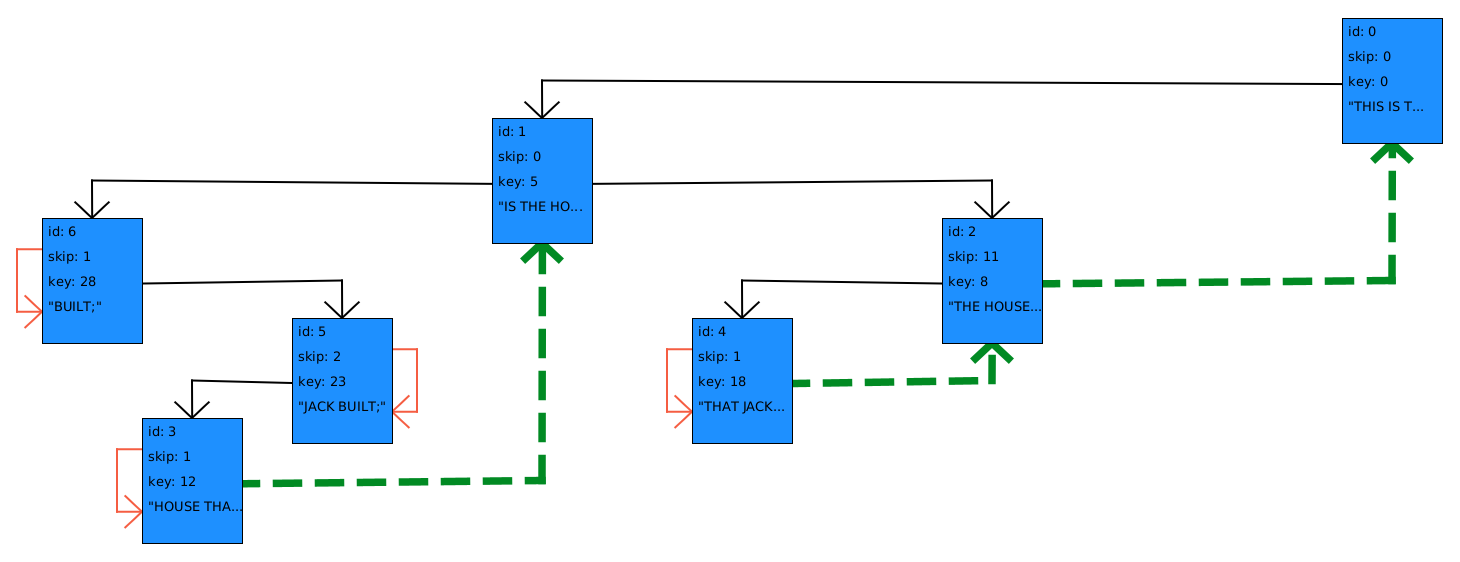
\includegraphics[width = \textwidth]{visaulRepresentation1.png}
    	\end{figure}
		
    	Główną klasą reprezentacji graficznej jest \emph{PatriciaTreeVisualRepresentation} w~paczce \emph{agh.jo.ui}. W implementacji głównej klasy i klas, z której korzysta, użyliśmy wtyczki (ang. \emph{plugin}) \emph{org.openjfx:javafx-maven-plugin:0.0.4} do \emph{Apache Maven 3.6.0}. Dodatkowo wykorzystaliśmy biblioteki \emph{org.openjfx:javafx-controls:13} oraz \emph{com.sirolf2009:fxgraph:0.0.3}. Rozszerzenia klas z tych bibliotek wykonaliśmy na podstawie przykładu podanego przez autora drugiej wymienionej biblioteki w popularnym serwisie \emph{StackOverflow} pod adresem \url{https://stackoverflow.com/questions/30679025/graph-visualisation-like-yfiles-in-javafx}.
		
		Reprezentacja graficzna była testowana manualnie na 7 przykładach struktury klasy \emph{PatriciaTree}. Część najciekawszych rezultatów testów manualnych została przedstawiona w postaci rysunków~ \ref{fig:PatriciaTreeVisualRepresentationTest1}, \ref{fig:PatriciaTreeVisualRepresentationTest2}, \ref{fig:PatriciaTreeVisualRepresentationTest3}, które znajdują się na następnej stronie.
		
        \begin{figure}[htb]
    		\caption{Przykładowa reprezentacja graficzna struktury klasy prostego przykładu \emph{PatriciaTree}, różniącego się od przykładu z~rysunku~\ref{fig:PatriciaTreeVisualRepresentation} jedynie wartościami parametrów wywołania konstruktora. Odmiennymi wartościami konstruktora klasy były: \emph{Encoding Encoding.JAVA} oraz \emph{WordStrategy WordStrategy.SINGLE}. Interpretacją wartości parametru konstruktora \emph{Encoding} jest fakt, iż klasa korzysta z~kodowania domyślnego \emph{JAVA} przy zamianie znaków na kod znaku i zamianie z kolei tego kodu na reprezentację binarną (o domyślnej długości bajtu równej 5 bitom). Interpretacją wartości parametru \emph{WordStrategy} jest przyjęcie strategii, gdzie klucz jest fragmentem pliku zaczynającego się w pozycji startowej klucza (przetrzymywanej w węźle drzewa w postaci pola \emph{key}) i kończącym się znakiem końca klucza, przed pozycją startową następnego klucza w pliku.}\label{fig:PatriciaTreeVisualRepresentationTest1}
    		\centering
    		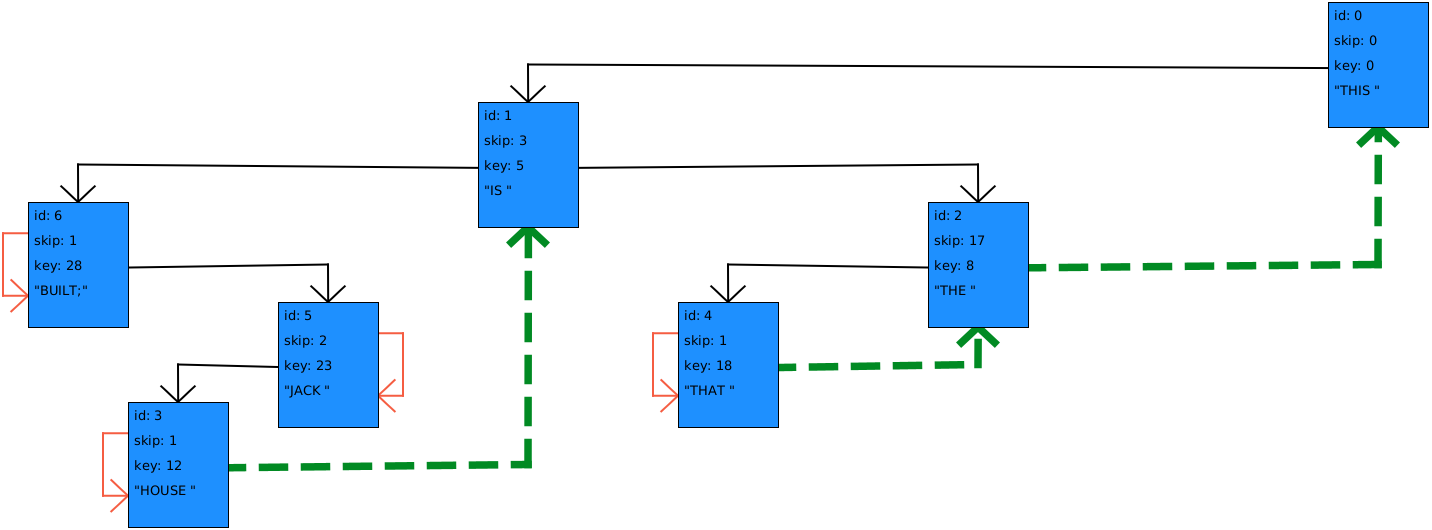
\includegraphics[width = \textwidth]{representationSmall_compressed.png}
    	\end{figure}
		
        \begin{figure}[htb]
    		\caption{Przykładowa reprezentacja graficzna struktury bardziej złożonego przykładu obiektu klasy \emph{PatriciaTree} różniącego się od przykładów przedstawionych na rysunkach~\ref{fig:PatriciaTreeVisualRepresentation} oraz~\ref{fig:PatriciaTreeVisualRepresentationTest1}. Widok przybliżony, przedstawia tą samą strukturę co rysunek~\ref{fig:PatriciaTreeVisualRepresentationTest3}.}\label{fig:PatriciaTreeVisualRepresentationTest2}
    		\centering
    		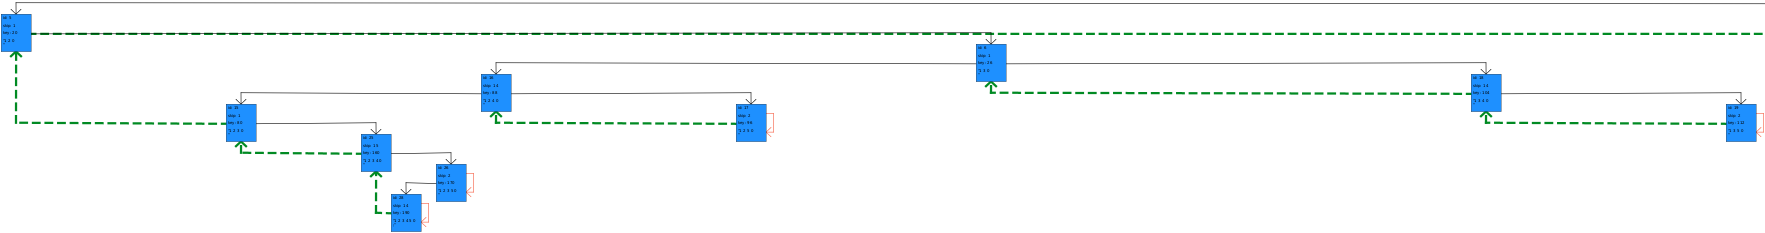
\includegraphics[width = \textwidth]{representationBigger-zoomedIn_compressed.png}
    	\end{figure}
    	
        \begin{figure}[htb]
    		\caption{Przykładowa reprezentacja graficzna struktury bardziej złożonego przykładu obiektu klasy \emph{PatriciaTree} różniącego się od przykładów przedstawionych na rysunkach \ref{fig:PatriciaTreeVisualRepresentation} oraz \ref{fig:PatriciaTreeVisualRepresentationTest1}. Widok oddalony, przedstawia tą samą strukturę co rysunek \ref{fig:PatriciaTreeVisualRepresentationTest2}.}\label{fig:PatriciaTreeVisualRepresentationTest3}
    		\centering
    		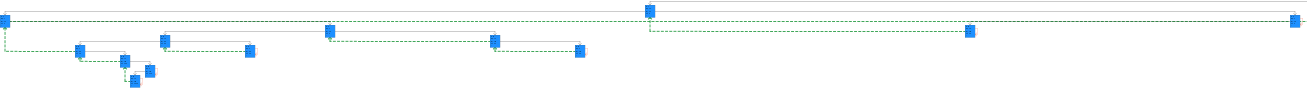
\includegraphics[width = \textwidth]{representationBigger-zoomedOut_compressed.png}
    	\end{figure}
		
		\section{Testy jednostkowe}\label{sec:czescPraktycznaRezultatyImplementacjiTestyJednostkowe}
		
    	Przez cały okres tworzenia i rozwijania autorskiej implementacji stopniowo dodawaliśmy testy jednostkowe pozwalające zweryfikować, czy nanoszone zmiany skutkowały spodziewanymi rezultatami. Mimo, że tworzenie ich zajęło nam bardzo dużo czasu, nie wyobrażam sobie, abyśmy bez nich byli w stanie znaleźć wiele pomyłek w naszym rozumowaniu, czy w tak efektywny sposób testować nasze podejrzenia co do trudniejszych do zrozumienia fragmentów algorytmów opisanych przez Knuth'a.
		
		Testy jednostkowe sprawdzają poprawność tworzonej struktury na różnych etapach, przy różnych konfiguracjach konstruktora klasy \emph{PatriciaTree} oraz na różnych przykładach plików źródłowych drzewa \emph{Patricia}. 
		
		W skład różnych testowanych etapów tworzenia struktury wchodzą między innymi: 
		\begin{enumerate}
		    \item Odczyt każdego ze znaków, 
		    \item Zamiana tego znaku na reprezentację binarną zgodną z wybranym kodowaniem,
		    \item Odczytywanie odpowiedniego fragmentu pliku zgodnie z przyjętą strategią.
		\end{enumerate}
		
		W skład testowanych konfiguracji konstruktora klasy \emph{PatriciaTree} wchodzą wszystkie możliwe kombinacje:
		\begin{enumerate}
		    \item Ilość bitów przyjętych dla symulowanej maszyny \emph{MIX},
		    \item Kodowanie znaków według tablicy znaków maszyny \emph{MIX} lub \emph{UTF-16},
		    \item Strategii: \emph{WordStrategy.SINGLE} lub \emph{WordStrategy.START\textunderscore POSITION \textunderscore TO\textunderscore EOF},
		    \item Różne kombinacje parametrów znaków \emph{charEOF} oraz \emph{charEOK},
		    \item Różne kombinacje konfiguracji konstruktora klasy \emph{CNFConverter}.
		\end{enumerate}
		
		W skład testowanych plików, na podstawie których tworzone są obiekty klasy \emph{PatriciaTree} wchodzi 7 plików źródłowych. Zawartość jednego z większych testowanych plików o rozmiarze 1.5 MB została przedstawiona fragmentem kodu źródłowego~\ref{prog:CNFsourceFile} oraz~\ref{prog:PatriciaSourceFile}. Drugi większy plik ma rozmiar 8.4 MB i na jego podstawie jest tworzony plik źródłowy drzewa \emph{Patricia}, którego zawartość przypomina plik w formacie \emph{DIMACS CNF}. Oznacza to, że plik wejściowy i wyjściowy konwertera różni się jedynie posortowanymi literałami wewnątrz klauzul, dodanym znakiem końca pliku ';', zamianą znaku końca linii na znak '\textbackslash n', brakiem linii komentarzy oraz linii problemu. Istnieje również trzeci plik w formacie \emph{DIMACS CNF} testujący współdziałanie klas \emph{CNFConverter} oraz \emph{PatriciaTree}, którego efektem jest reprezentacja wizualna z rysunków~\ref{fig:PatriciaTreeVisualRepresentationTest2} oraz~\ref{fig:PatriciaTreeVisualRepresentationTest3}. Dodatkowo stworzyliśmy 6 plików na podstawie zmodyfikowanego przykładu omawianego przez Knuth'a w swojej książce~\cite{KnuthsTheArtOfComputerProgramming3}. Treść tych plików wygląda następująco:
		\begin{enumerate}
		    \item \texttt{THIS IS THE HOUSE THAT JACK BUILT;}
		    \item \texttt{THIS$\Phi$IS$\Phi$THE$\Phi$HOUSE$\Phi$THAT$\Phi$JACK$\Phi$BUILT$\Phi\Pi$}
		    \item \texttt{THIS$\Phi$IS$\Phi\Phi$THE$\Phi$HOUSE$\Phi$THAT$\Phi$JACK$\Phi$BUILT$\Phi\Phi\Phi\Phi\Pi$ This Is Not A Part Of Any Key Because Of EOF Character $\Pi$}
		    \item \texttt{THIS $\Phi$IS $\Phi\Phi$THE $\Phi$HOUSE $\Phi$THAT $\Phi$JACK $\Phi$BUILT ;$\Phi\Phi\Phi\Phi\Pi$ This Is Not A Part Of Any Key Because Of EOF Character $\Pi$}
		    \item \texttt{THIS IS THE TEST FILE NUMBER 1 FOR DELETION ONE OF NODES. LONGESTWORDINTREE TODELETE. MORE NODES AFTER NODE TO DELETE;}
		    \item \texttt{THIS IS THE TEST FILE NUMBER 1 FOR DELETION ONE OF NODES. LONGESTWORDINTREExTODELETE. MORE NODES AFTER NODE TO DELETE;}
		\end{enumerate}
        
        Z dumą możemy powiedzieć, że wyżej omówione testy pokrywają następujący zakres klas, metod oraz linii kodu:
    
        \begin{enumerate}
            \item Względem głównej paczki (ang. \emph{package}) jaką jest \emph{agh.jo}:
                \subitem Pokrycie klas: 43\%,
                \subitem Pokrycie metod: 50\%,
                \subitem Pokrycie linii kodu: 45\%;
            \begin{enumerate}
                \item Względem paczki \emph{agh.jo.cnf.converter} (zawierającą klasy odpowiadające za przetwarzanie pliku w formacie .cnf):
                    \subitem Pokrycie klas: 100\%,
                    \subitem Pokrycie metod: 88\%,
                    \subitem Pokrycie linii kodu: 94\%;
                \item Względem paczki \emph{agh.jo.knuth} (zawierającą klasy związane ściśle z implementacją drzewa \emph{Patricia}):
                    \subitem Pokrycie klas: 100\%,
                    \subitem Pokrycie metod: 88\%,
                    \subitem Pokrycie linii kodu: 80\%;
                \item Względem paczki \emph{agh.jo.ui} (zawierającą klasy związane z reprezentacją graficzną struktury drzewa \emph{Patricia}):
                    \subitem Pokrycie klas: 0\%,
                    \subitem Pokrycie metod: 0\%,
                    \subitem Pokrycie linii kodu: 0\%;
                \item Względem paczki \emph{utils} (zawierającą klasy używane w wielu innych paczkach, na przykład te odpowiadające za obsługę klasy \emph{RandomAccessFile}):
                    \subitem Pokrycie klas: 60\%,
                    \subitem Pokrycie metod: 75\%,
                    \subitem Pokrycie linii kodu: 63\%.
            \end{enumerate}
        \end{enumerate}
	
    	\section{Instrukcja uruchomienie programu inżynierskiego}\label{sec:czescPraktycznaUruchamianieProgramu}
    	
    	Program inżynierski został napisany w sposób pozwalający na uruchomienie go w~kilku wariantach. Decyzja podziału na kilka wariantów uruchamiania spowodowana była długim czasem wykonywania i brakiem przejrzystości, gdy wszystkie warianty programu zostawały uruchomione jeden po drugim. 
    	
    	Uruchomienie podstawowej funkcjonalności programu odbywa się po przez przejście do folderu zawierającego foldery \emph{target} oraz \emph{src} i wpisaniu w konsoli komendy przedstawionej w postaci kodu źródłowego \ref{prog:runProgramJar}.
    	
    	\begin{program}
			\caption{Komenda pozwalającą uruchomić program w postaci pliku wykonywalnego \emph{jar} będąc w folderze zawierającym foldery \emph{target} oraz \emph{src}.}\label{prog:runProgramJar}
			\begin{lstlisting}[basicstyle=\small,]
java -jar target/TrieTreeImplementations_complete_standalone.jar RUN_MODE EXAMPLE_NUMBER OPTIONAL_DO_CONVERT_CNF_FILE
    	    \end{lstlisting}
	    \end{program}
    	
    	Zawartością folderu \emph{target} jest plik wykonywalny w formacie \emph{jar}. Konsekwencją zawarcia programu w postaci pliku wykonywalnego jest konieczność zawarcia dodatkowych plików, na których program przeprowadza operacje w oddzielnym folderze \emph{src/main/resources}. Są to pliki w formacie tekstowym o rozszerzeniu \emph{.cnf} lub \emph{.txt}. Pliki \emph{.cnf} są wykorzystywane przy konwersji ich do plików \emph{.txt}, które z kolei używane są do budowy struktury drzew \emph{Patricia} zawartych w postaci obiektów klasy \emph{PatriciaTree}.
    	
    	Komenda uruchamiająca plik wykonywalny, przedstawiona kodem źródłowym \ref{prog:runProgramJar} przyjmuje 3 parametry jako argumenty przedstawianego programu. 
    	\begin{enumerate}
    	    \item Pierwszym argumentem jest tryb w jakim chcielibyśmy uruchomić program - \texttt{RUN\textunderscore MODE}: 
    	        \subitem tekstowy -- dla którego wartość parametru powinna być równa \texttt{text};\newline
    	        Jest to tryb w którym informacje na temat drzewa przedstawiane są postaci tekstowej. Krótkie przykłady wyświetlają informacje o poszczególnych kluczach oraz prefiksach drzewa. Długie przykłady ze względu na czytelność tego rozwiązania nie robią tego. Oprócz tego, jeżeli dany przykład ma taką możliwość i zdecydujemy się na to, wyświetlana jest również informacja o dokonaniu konwersji pliku \emph{CNF} na plik źródłowy drzewa \emph{Patricia} (oczywiście przed jego stworzeniem).
    	        \subitem graficzny -- dla którego wartość parametru powinna być równa \texttt{visual};\newline
    	        Jest to tryb reprezentacji graficznej struktury drzewa zawartej w postaci obiektu klasy \emph{PatriciaTree}. Wykonuje on operacje opisane w trybie tekstowym oraz na ich koniec przedstawia użytkownikowi wizualizację stworzonego drzewa \emph{Patricia}.
    	   \item Drugim argumentem jest numer przykładu jaki chcielibyśmy, aby program przedstawił -- \texttt{EXAMPLE\textunderscore NUMBER}:
    	        \subitem Przyjmuje on jako swoje wartości liczby całkowite z zakresu od $0$ do $9$ odpowiadające indeksowi przykładu. \newline
    	        
            	Przykłady o numerach indeksów $5$ i $6$ są zbyt duże, aby obecna implementacja reprezentacji graficznej sobie z nimi poradziła, dlatego są one zabezpieczone wyjątkiem niepozwalającym na uruchomienie ich w trybie uruchomienia \texttt{visual}.
    	        \begin{enumerate}[label*=\arabic*.]
    	            \setcounter{enumii}{-1}
    	            \item Wartość \texttt{0} odpowiada przykładowi o indeksie $0$.
    	                \begin{enumerate}
    	                    \item Kodowanie znaków jest zgodne z kodowanie znaków w symulowanej maszynie \emph{MIX}.
    	                    \item Strategia pobierania kluczy definiująca czym jest znak jest równa \emph{START\textunderscore POSITION\textunderscore TO\textunderscore EOF}.
    	                    \item Nie zawiera pliku zawierającego koniunkcyjną postać normalną.
    	                    \item Zawartością pliku źródłowego obiektu klasy \emph{PatriciaTree} mu odpowiadającego jest: \newline
    	                ,,\texttt{THIS IS THE HOUSE THAT JACK BUILT;}``
    	                    \item Dodatkowo w pracy można zobaczyć wynik reprezentacji graficznej dla tego przykładu w postaci figury \ref{fig:PatriciaTreeVisualRepresentation}.
    	                \end{enumerate}
    	                
    	            \item Wartość \texttt{1} odpowiada przykładowi o indeksie $1$.
    	                \begin{enumerate}
    	                    \item Kodowanie znaków jest zgodne z kodowanie znaków w wirtualnej maszynie języka \emph{Java}.
    	                    \item Strategia pobierania kluczy definiująca czym jest znak jest równa \emph{SINGLE}.
    	                    \item Nie zawiera pliku zawierającego koniunkcyjną postać normalną.
    	                    \item Zawartością pliku źródłowego obiektu klasy \emph{PatriciaTree} mu odpowiadającego jest: \newline
    	                ,,\texttt{THIS IS THE HOUSE THAT JACK BUILT;}``
    	                    \item Dodatkowo w pracy można zobaczyć wynik reprezentacji graficznej dla tego przykładu w postaci figury \ref{fig:PatriciaTreeVisualRepresentationTest1}.
    	                \end{enumerate}
    	                
    	            \item Wartość \texttt{2} odpowiada przykładowi o indeksie $2$.
    	                \begin{enumerate}
    	                    \item Kodowanie znaków jest zgodne z kodowanie znaków w wirtualnej maszynie języka \emph{Java}.
    	                    \item Strategia pobierania kluczy definiująca czym jest znak jest równa \emph{SINGLE}.
    	                    \item Nie zawiera pliku zawierającego koniunkcyjną postać normalną.
    	                    \item Zawartością pliku źródłowego obiektu klasy \emph{PatriciaTree} mu odpowiadającego jest: \newline
    	                ,,\texttt{THIS$\Phi$IS$\Phi$THE$\Phi$HOUSE$\Phi$THAT$\Phi$JACK$\Phi$BUILT$\Phi\Pi$}``
    	                \end{enumerate}
    	                
    	            \item Wartość \texttt{3} odpowiada przykładowi o indeksie $3$.
    	                \begin{enumerate}
    	                    \item Kodowanie znaków jest zgodne z kodowanie znaków w wirtualnej maszynie języka \emph{Java}.
    	                    \item Strategia pobierania kluczy definiująca czym jest znak jest równa \emph{SINGLE}.
    	                    \item Nie zawiera pliku zawierającego koniunkcyjną postać normalną.
    	                    \item Zawartością pliku źródłowego obiektu klasy \emph{PatriciaTree} mu odpowiadającego jest: \newline
    	                ,,\texttt{THIS$\Phi$IS$\Phi\Phi$THE$\Phi$HOUSE$\Phi$THAT$\Phi$JACK$\Phi$BUILT$\Phi\Phi\Phi\Phi\Pi$ This Is Not A Part Of Any Key Because Of EOF Character $\Pi$}``
    	                \end{enumerate}
    	                
    	            \item Wartość \texttt{4} odpowiada przykładowi o indeksie $4$.
    	                \begin{enumerate}
    	                    \item Kodowanie znaków jest zgodne z kodowanie znaków w wirtualnej maszynie języka \emph{Java}.
    	                    \item Strategia pobierania kluczy definiująca czym jest znak jest równa \emph{SINGLE}.
    	                    \item Nie zawiera pliku zawierającego koniunkcyjną postać normalną.
    	                    \item Zawartością pliku źródłowego obiektu klasy \emph{PatriciaTree} mu odpowiadającego jest: \newline
    	                ,,\texttt{THIS $\Phi$IS $\Phi\Phi$THE $\Phi$HOUSE $\Phi$THAT $\Phi$JACK $\Phi$BUILT ;$\Phi\Phi\Phi\Phi\Pi$ This Is Not A Part Of Any Key Because Of EOF Character $\Pi$}``
    	                \end{enumerate}
    	                
    	            \item Wartość \texttt{5} odpowiada przykładowi o indeksie $5$.
    	                \begin{enumerate}
    	                    \item Kodowanie znaków jest zgodne z kodowanie znaków w wirtualnej maszynie języka \emph{Java}.
    	                    \item Strategia pobierania kluczy definiująca czym jest znak jest równa \emph{SINGLE}.
    	                    \item Plik zawierający koniunkcyjną postać normalną ma rozmiar 1,5 Mb, a~fragment jego zawartości przedstawia kod źródłowy \ref{prog:CNFsourceFile}.
    	                    \item Plik źródłowy obiektu klasy \emph{PatriciaTree} ma rozmiar 1,5 Mb, a jego fragment przestawia kod źródłowy \ref{prog:PatriciaSourceFile}.
    	                \end{enumerate}
    	                
    	            \item Wartość \texttt{6} odpowiada przykładowi o indeksie $6$.
    	                \begin{enumerate}
    	                    \item Kodowanie znaków jest zgodne z kodowanie znaków w wirtualnej maszynie języka \emph{Java}.
    	                    \item Strategia pobierania kluczy definiująca czym jest znak jest równa \emph{SINGLE}.
    	                    \item Plik zawierający koniunkcyjną postać normalną ma rozmiar 8,4 Mb, a~jego zawartość przypomina strukturę pliku \emph{CNF} przykładu o indeksie $5$.
    	                    \item Plik źródłowy obiektu klasy \emph{PatriciaTree} ma rozmiar 8,4 Mb, a jego zawartość jest zbliżona do zawartości pliku \emph{CNF} tego przykładu (o indeksie $6$). Rozróżnia go zakończenie każdej linii w postaci znaku '\textbackslash n', znak końca pliku postaci znaku ';', posortowane literały w każdej z klauzul oraz brak linii komentarzy oraz linii problemu.
    	                \end{enumerate}
    	                
    	            \item Wartość \texttt{7} odpowiada przykładowi o indeksie $6$.
    	                \begin{enumerate}
    	                    \item Kodowanie znaków jest zgodne z kodowanie znaków w wirtualnej maszynie języka \emph{Java}.
    	                    \item Strategia pobierania kluczy definiująca czym jest znak jest równa \emph{SINGLE}.
    	                    \item Plik zawierający koniunkcyjną postać normalną ma rozmiar 532 bajtów, a~jego zawartość przypomina strukturę innych plików \emph{CNF} (z przykładów o indeksie $5$ i $6$).
    	                    \item Plik źródłowy obiektu klasy \emph{PatriciaTree} ma rozmiar 203 bajtów, a jego zawartość jest zbliżona do zawartości pliku \emph{CNF} tego przykładu (o indeksie $7$). \newpage Rozróżnia go zakończenie każdej linii w postaci znaku '\textbackslash n', znak końca pliku postaci znaku ';', posortowane literały w każdej z klauzul oraz brak linii komentarzy oraz linii problemu.
    	                    \item Dodatkowo w pracy można zobaczyć wynik reprezentacji graficznej dla tego przykładu w postaci figur \ref{fig:PatriciaTreeVisualRepresentationTest2} i \ref{fig:PatriciaTreeVisualRepresentationTest3}.
    	                \end{enumerate}
    	                
    	            \item Wartość \texttt{8} odpowiada przykładowi o indeksie $8$.
    	                \begin{enumerate}
    	                    \item Kodowanie znaków jest zgodne z kodowanie znaków w wirtualnej maszynie języka \emph{Java}.
    	                    \item Strategia pobierania kluczy definiująca czym jest znak jest równa \emph{SINGLE}.
    	                    \item Nie zawiera pliku zawierającego koniunkcyjną postać normalną.
    	                    \item Zawartością pliku źródłowego obiektu klasy \emph{PatriciaTree} mu odpowiadającego jest: \newline
    	                ,,\texttt{THIS IS THE TEST FILE NUMBER 1 FOR DELETION ONE OF NODES. LONGESTWORDINTREE TODELETE. MORE NODES AFTER NODE TO DELETE;}``
    	                    \item Dodatkowo w pracy można zobaczyć wynik reprezentacji graficznej dla tego przykładu w postaci figury \ref{fig:Delete1}.
    	                \end{enumerate}
    	                
    	            \item Wartość \texttt{9} odpowiada przykładowi o indeksie $9$.
    	                \begin{enumerate}
    	                    \item Kodowanie znaków jest zgodne z kodowanie znaków w wirtualnej maszynie języka \emph{Java}.
    	                    \item Strategia pobierania kluczy definiująca czym jest znak jest równa \emph{SINGLE}.
    	                    \item Nie zawiera pliku zawierającego koniunkcyjną postać normalną.
    	                    \item Zawartością pliku źródłowego obiektu klasy \emph{PatriciaTree} mu odpowiadającego jest: \newline
    	                ,,\texttt{THIS IS THE TEST FILE NUMBER 1 FOR DELETION ONE OF NODES. LONGESTWORDINTREExTODELETE. MORE NODES AFTER NODE TO DELETE;}``
    	                    \item Dodatkowo w pracy można zobaczyć wynik reprezentacji graficznej dla tego przykładu w postaci figury \ref{fig:Delete2}.
    	                \end{enumerate}
    	        \end{enumerate}
    	    \item Trzecim argumentem jest opcjonalny argument decydujący o tym czy przed stworzeniem obiektu klasy \emph{PatriciaTree} chcielibyśmy wykonać konwersję pliku \emph{CNF} na źródłowy dla naszego obiektu -- \texttt{OPTIONAL\textunderscore DO\textunderscore CONVERT\textunderscore CNF\textunderscore FILE}. Przyjmuje wartość \texttt{true} lub \texttt{false}. \newline 
    	    
    	    Pliki źródłowe obiektów klasy \emph{PatriciaTree} dla wszystkich przykładów są stworzone przed uruchomieniem programu. Nie należy ich kasować. Można wykasować ich zawartość. Są one nadpisywane w przypadku, gdy argument ten przyjmuje wartość \texttt{true}. Gdy nie zostanie podany ten parametr, domyślną przyjmowaną wartością jest \emph{false} wewnątrz programu.
    	\end{enumerate}